\chapter{DC Circuits}

% Triplett 9007 (often blown fuse)
% Mastech MS8264 (resettable fuse)
% Wish Board No.  206
% MASTECH HY3005F-3

\section{Introduction}

In this lab, you will learn how to use your digital multimeter (DMM)
and bench-top DC power supply to explore DC circuits involving
resistors.  You will experimentally verify Ohm's law and the
equivalent resistance for resistors in series and parallel.

If time permits, you will also solder two resistor circuits to explore
the $\Delta$-$Y$ transformation for three terminal networks.

\section{Benchtop Power Supply}

\begin{figure}[htbp]
\begin{center}
\begin{tikzpicture}
    \node[anchor=south west,inner sep=0] (image) at (0,0,0) {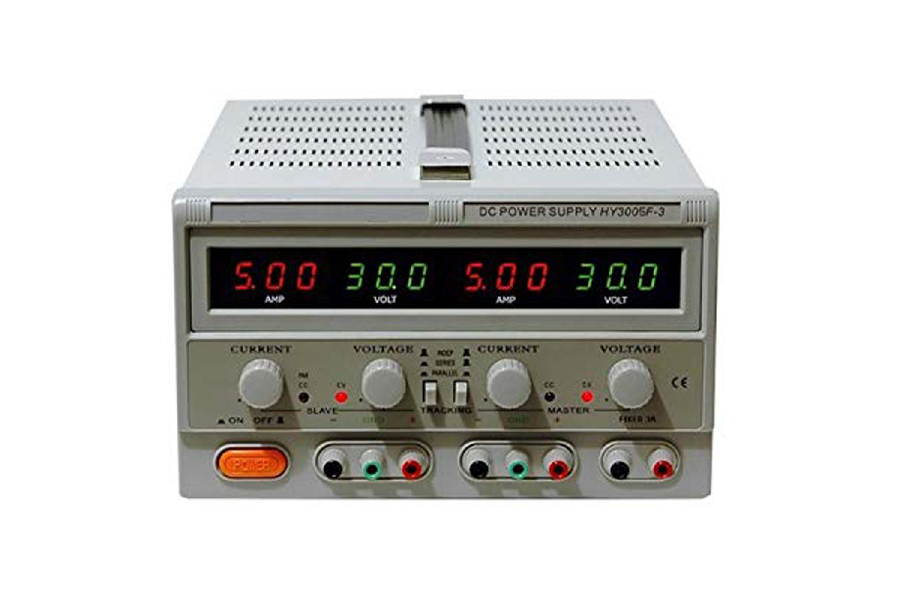
\includegraphics[height=0.40\textheight]{figs/labs/dc_circuits/dc_supply.pdf}};
    \node[right](X) at (0,5.0) {Voltage};
    \draw (X.east) -- (6.2,3.5);
    \node[right](X) at (0,3.0) {Current};
    \draw (X.east) -- (4.2,3.5);

    \node[right](X) at (0,2.0) {LED};
    \draw (X.east) -- (5.35,3.3);
    \node[right](X) at (0,0) {Power};
    \draw (X.east) -- (3.9,2.1);

    \node[right](X) at (3,0) {Negative};
    \draw (X.north) -- (5.3,2.1);

    \node[right](X) at (5,0) {Ground};
    \draw (X.north) -- (6.0,2.1);

    \node[right](X) at (7,0) {Positive};
    \draw (X.north) -- (6.7,2.1);

    \node[right](X) at (9,0) {Push Button};
    \draw (X.north) -- (6.9,3.4);

    \node[left](X) at (14,7) {Display};
    \draw (X.west) -- (10,5);

    %\node[](C) at (0,1) {Current};
    %\node[](D) at (0,3) {Voltage};
\end{tikzpicture}
\caption{Your bench-top DC power supply, the MASTECH 3005F-3.}
\label{fig:dcsupply}
\end{center}
\end{figure}

In this lab you will use one channel of your MASTECH 3005F-3 DC
power-supply as the voltage source in your experimental circuits.  See
Fig.~\ref{fig:dcsupply} for the location of the control features.
Since you won't know initially what settings your power-supply was
left at, leave the supply disconnected while you configure the supply
to provide $10~\rm V$.

First, check that the supply is set to provide two independent outputs
(you will only use one for this lab) by making sure both bush buttons
are out.  Next, power the device by pressing the power button.  Your
power supply has both a current limit knob and a voltage limit knob.
Usually, we specify the voltage you want in your circuit, but even in
this case, the current limit is useful for protecting your circuit and
measurement equipment.  When the LED labeled ``CV'' is lit, the
voltage limit is controlling the output.  When the LED labeled ``CC''
is lit, the current limit is controlling the output.

Turn the voltage limit knob clockwise and watch the voltage increase
on the display.  If the CC LED lights, it indicates that the current
limit is active, and you will not be able to raise the voltage.  Turn
the current limit knob until just a bit after the CV LED lights,
indicating the voltage limit is active.  Continue raising the voltage
until you reach the $10~\rm V$.  Once you reach your target voltage,
turn the current limit counter-clockwise, to lower the current limit,
until the LED labeled ``CC'' lights, indicated you have reached the
current limit.  Turn the current limit clockwise just past the point
that the device goes back to being voltage limited.  If you get in the
habit of doing this every time you use your bench-top supply, you will
safe many components for accidental damage!

The voltage on the display is maintained between the black (-)
terminal and the red (+) terminal.  It is floating, meaning that only
the difference is set by the device, just like a battery, and you may
connect ground wherever you choose (within the limits of the supply).
If you wish to provide a ground referenced DC voltage, you connect the
green terminal to the appropriate terminal.  For example, connecting
green to red would provide $-10~\rm V$ referenced to ground at the
negative terminal.  You will leave the supply floating for this
experiment.

\section{Voltage Measurement}

\begin{figure}[htbp]
\begin{center}
\begin{tabular}{cc}
\begin{tikzpicture}
    \node[anchor=center,inner sep=0] (image) at (0,0,0) {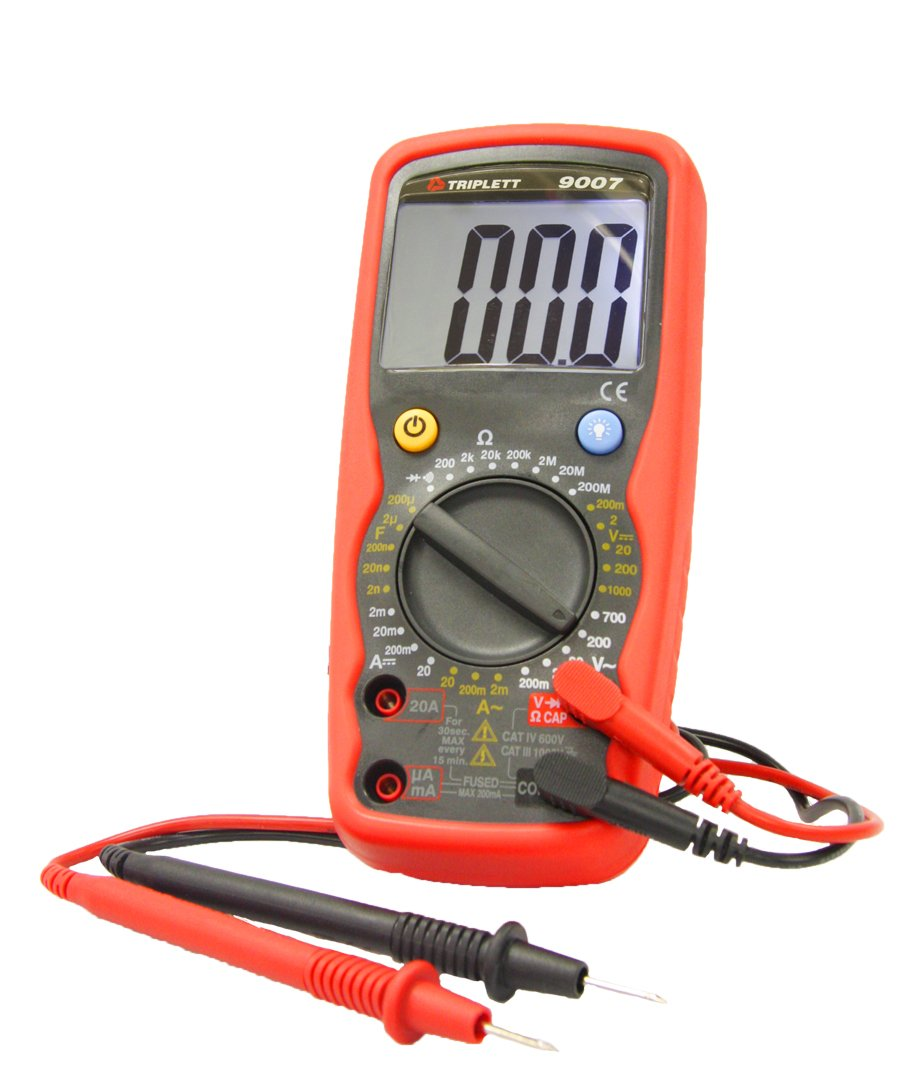
\includegraphics[height=0.35\textheight]{figs/labs/dc_circuits/triplett.jpg}};

    \node[right](X) at (-5.,2.0) {Power};
    \draw (X.east) -- (-0.25,1);

    \node[right](X) at (-5.,-1.0) {Current};
    \draw (X.east) -- (-0.6,-1.8);

    \node[right](X) at (-5.,-4.0) {Probes};
    \draw (X.east) -- (-2.,-3.0);

    \node[left](X) at (5.,-4.0) {Common};
    \draw (X.west) -- (1.0,-2.0);

    \node[left](X) at (5.,-1.0) {Voltage};
    \draw (X.west) -- (1.0,-1.0);

    \node[left](X) at (5.,1.0) {Dial};
    \draw (X.west) -- (0.3,-0.25);

\end{tikzpicture}&
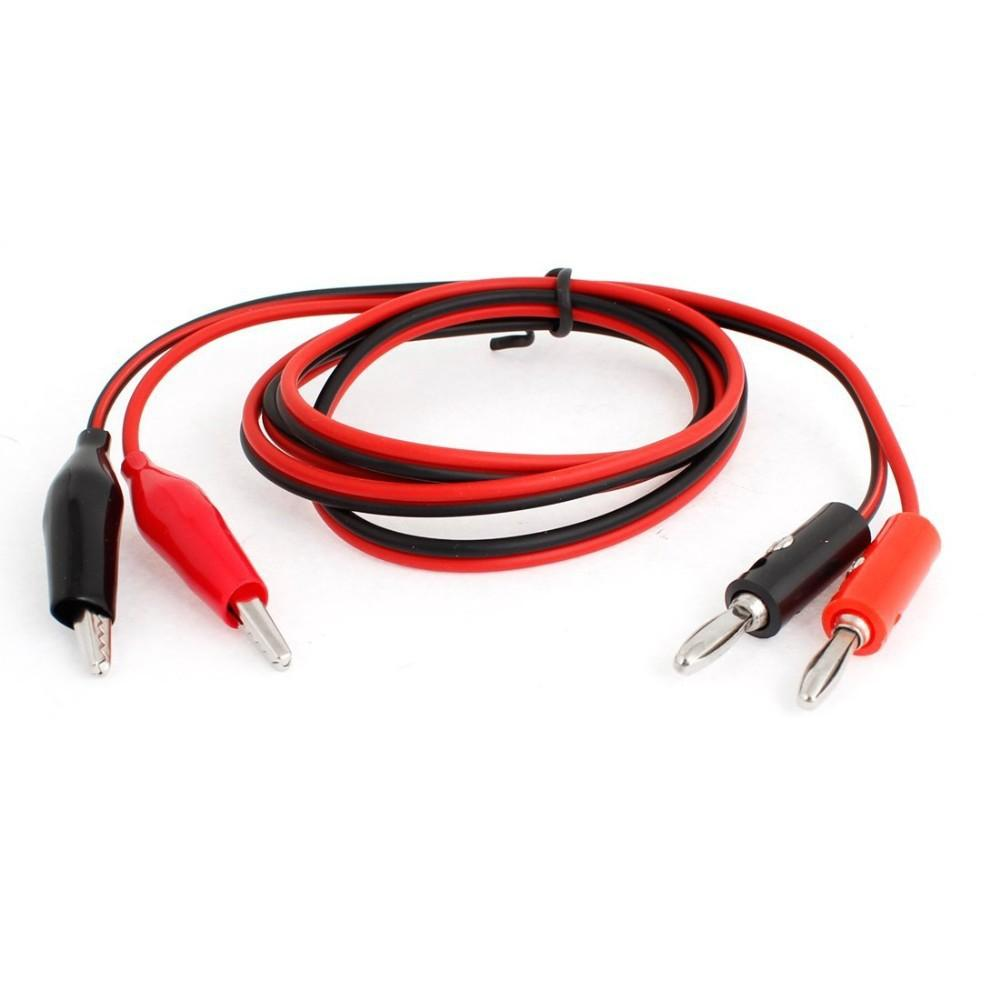
\includegraphics[height=0.2\textheight]{figs/labs/dc_circuits/alligator.jpg}
\\
(a) & (b) \\
\end{tabular}
\caption{Your (a) digital multimeter (DMM), the Triplett 9007, and (b) alligator clip probes.}
\label{fig:triplett}
\end{center}
\end{figure}

Your primary digital multimeter (DMM), the Triplett 9007 shown in
Fig~\ref{fig:triplett}, can be used to make a number of measurements
including resistance, DC current, and DC voltage.  We'll measure a DC
voltage to start.  This lab will be most convenient if you use
alligator clip probes in your DMM.  Install a black alligator clip
probe in the ``Common'' terminal, and a red alligator clip probe in
the ``Voltage'' terminal directly above the Common terminal.  Clip the
alligator clips together so that you expect to measure $0~\rm V$.  Now
power the DMM by pressing the power button, and turn the voltage dial
to the DC voltage measurement, the $V$ with one straight and one
dashed line next to it.  Most measurements on your DMM have a number
of different full range settings.  For the highest precision, you
should use the smallest full-range setting larger than your
measurement.  We'll be measuring $10~\rm V$, so use the $20~\rm V$
(DC) setting.

With the alligator clip probes connected together, your DMM should
read $0.00~\rm V$.  Now touch the probes to the terminals on your
bench-top DC voltage supply: red probe to red terminal, and black
probe to black terminal.  You should read $10~\rm V$.  Next touch red
probe to black terminal and black probe to red terminal.  You should
read $-10~\rm V$.  This is because the ``Common'' (black) probe is the
reference point for the measurement, and the red probe is currently
connected to a point $10~\rm V$ lower than this reference point.

\section{Resistance Measurement}

\begin{figure}[htbp]
\begin{center}
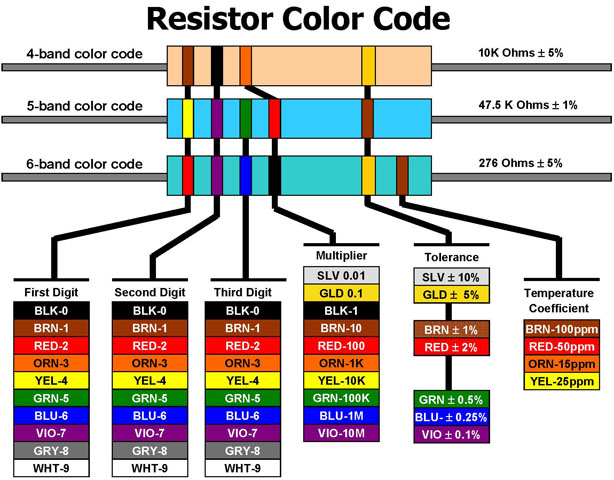
\includegraphics[height=0.45\textheight]{figs/labs/dc_circuits/rcolor.jpg}
\caption{The resistor color code.}
\label{fig:rcolor}
\end{center}
\end{figure}

Pick two different resistors from the random collection of resistors
at the front of the lab.  Connect the alligator clip across one of the
resistors, and turn the dial to the resistance measurement, marked
$\Omega$.  When the measurement reads ``1'' the resistance is larger
than the full range.  Find the smallest range larger than your
resistor and record the measured value.  Using the resistor color
coding guide in Fig.~\ref{fig:rcolor}, determine the nominal
resistance of your selected resistor.  In your logbook, record your
resistor color pattern, the nominal value you determined, and the
measured value.  Repeat this for a second resistor.


\section{Current Measurement}

\begin{figure}[htbp]
\begin{center}
\begin{tabular}{c@{\hskip 2cm}c}

\begin{circuitikz}[line width=1pt]
\draw (0,0) to[voltage source,bipoles/length=1.5cm] ++(0,+4.0) to[short] ++(2.0,0) coordinate(A);
\draw (A) to[resistor,l_=$R_1$] ++(0,-2.0) to[short] ++(0,-2.0) to[short] ++(-2,0);
\draw (A) to[short,*-] ++(2.0,0.0) to[short] ++(0.0,-1.0) node[component]{V} to[short] ++(0.0,-1.0) to[short,-*] 
++(-2.0,0);
\end{circuitikz} &

\begin{circuitikz}[line width=1pt]
\draw (0,0) coordinate(X) to[voltage source,bipoles/length=1.5cm] ++(0,+4.0) to[short] ++(2.0,0)
to[resistor,l_=$R_1$] ++(0,-2.0) to[short] ++(0,-1.0) node[component]{A} to[short] ++(0,-1.0) to[short] ++(-2.0,0);
\end{circuitikz} \\
(a) & (b) \\
\end{tabular}
\caption{Appropriate connections for measuring (a) the voltage across resistor $R_1$ and (b) the current through the resistor $R_1$.}
\label{fig:dmmconnect}
\end{center}
\end{figure}

Your DMM is designed to have minimal impact on the circuit your are
measuring.  When used to measure the voltage across a component, such
as a resistor, it is connected in parallel, as in
Fig.~\ref{fig:dmmconnect}a.  The ideal voltmeter therefore has
infinite resistance, so that no current from the circuit is diverted
through the voltmeter.  Your DMM has a $10~{\rm M\Omega}$ resistance
when used as a voltmeter.

When used to measure the current through a component, your DMM is
connected in series, allowing the current to pass through the device.
The ideal ammeter therefore has zero resistance, so that there is no
voltage drop across the voltmeter.  For this reason, most DMMs have
separate terminals for measuring currents. 

You make a current measurement with a DMM by installing the red probe
in a current terminal (instead of the voltage terminal) the black
probe in the common terminal as before, and installing the probe in
series with the component you wish to measure the current through.

However, the current measurement in your Triplett 9007 is fused, and
you can fairly safely assume that the fuse is blown.  Because the
current measurement is nearly a short circuit, it is very easy to
introduce an unintentionally large current by connecting a voltage
across the terminals, as if to measure a voltage.  Even experience is no
sure remedy for this common lab mishap.

Instead, we will use the Mastech MS8264 which features a resettable
fuse for making current measurements.

\section{Breadboard}

\begin{figure}[htbp]
\begin{center}
\begin{tikzpicture}
    \node[anchor=center,inner sep=0] (image) at (0,0,0) {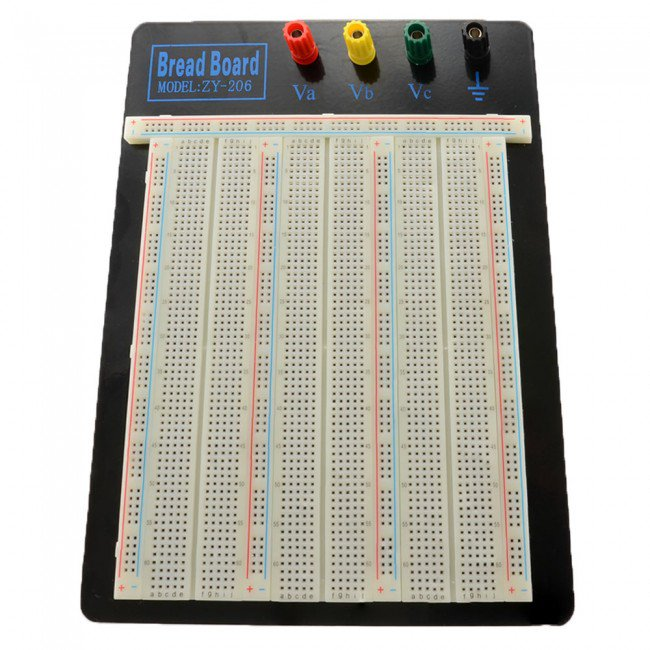
\includegraphics[height=0.35\textheight]{figs/labs/dc_circuits/breadboard.jpg}};

    \node[left](X) at (6.,2.0) {Terminal Strip};
    \draw (X.west) -- (1.2,1.0);
    \draw (1.0,1.0) -- (1.4,1.0);

    \node[right](X) at (-5.,-1.0) {Bus Strip};
    \draw (X.east) -- (-0.765,-0.55);
    \draw (-0.85,-3.3) -- (-0.68,2.2);

\end{tikzpicture}
\caption{A typical breadboard.}
\end{center}
\end{figure}

Breadboards are a convenient way to prototype circuits without having
to solder.  When the leads of discrete components are inserted in the
holes in the breadboard, they make electrical contact with metal
strips inside the breadboard that connect with additional holes.  
The short terminal strips are used to make electrical connections
between components.  The longer bus strips are a convenient way to
bring in ground or voltage supplies that need to connect to many
places in circuit.

\section{Verification of Ohm's Law}

\begin{figure}[htbp]
\begin{center}
\begin{tabular}{c@{\hskip 2cm}c}

\begin{circuitikz}[line width=1pt]
\draw (0,0) to[voltage source,bipoles/length=1.5cm] ++(0,+4.0) to[short] ++(2.0,0) coordinate(A);

\draw (A) to[resistor,l_=$R_1$] ++(0,-2.0) to[short] ++(0,-1.0) 
node[component]{A} to[short] ++(0,-1.0) to[short] ++(-2.0,0);
%node[ground,yscale=2.0]{};
\draw (A) to[short,*-] ++(2.0,0.0) to[short] ++(0.0,-1.0) node[component]{V} to[short] ++(0.0,-1.0) to[short,-*] 
++(-2.0,0);
\end{circuitikz} &
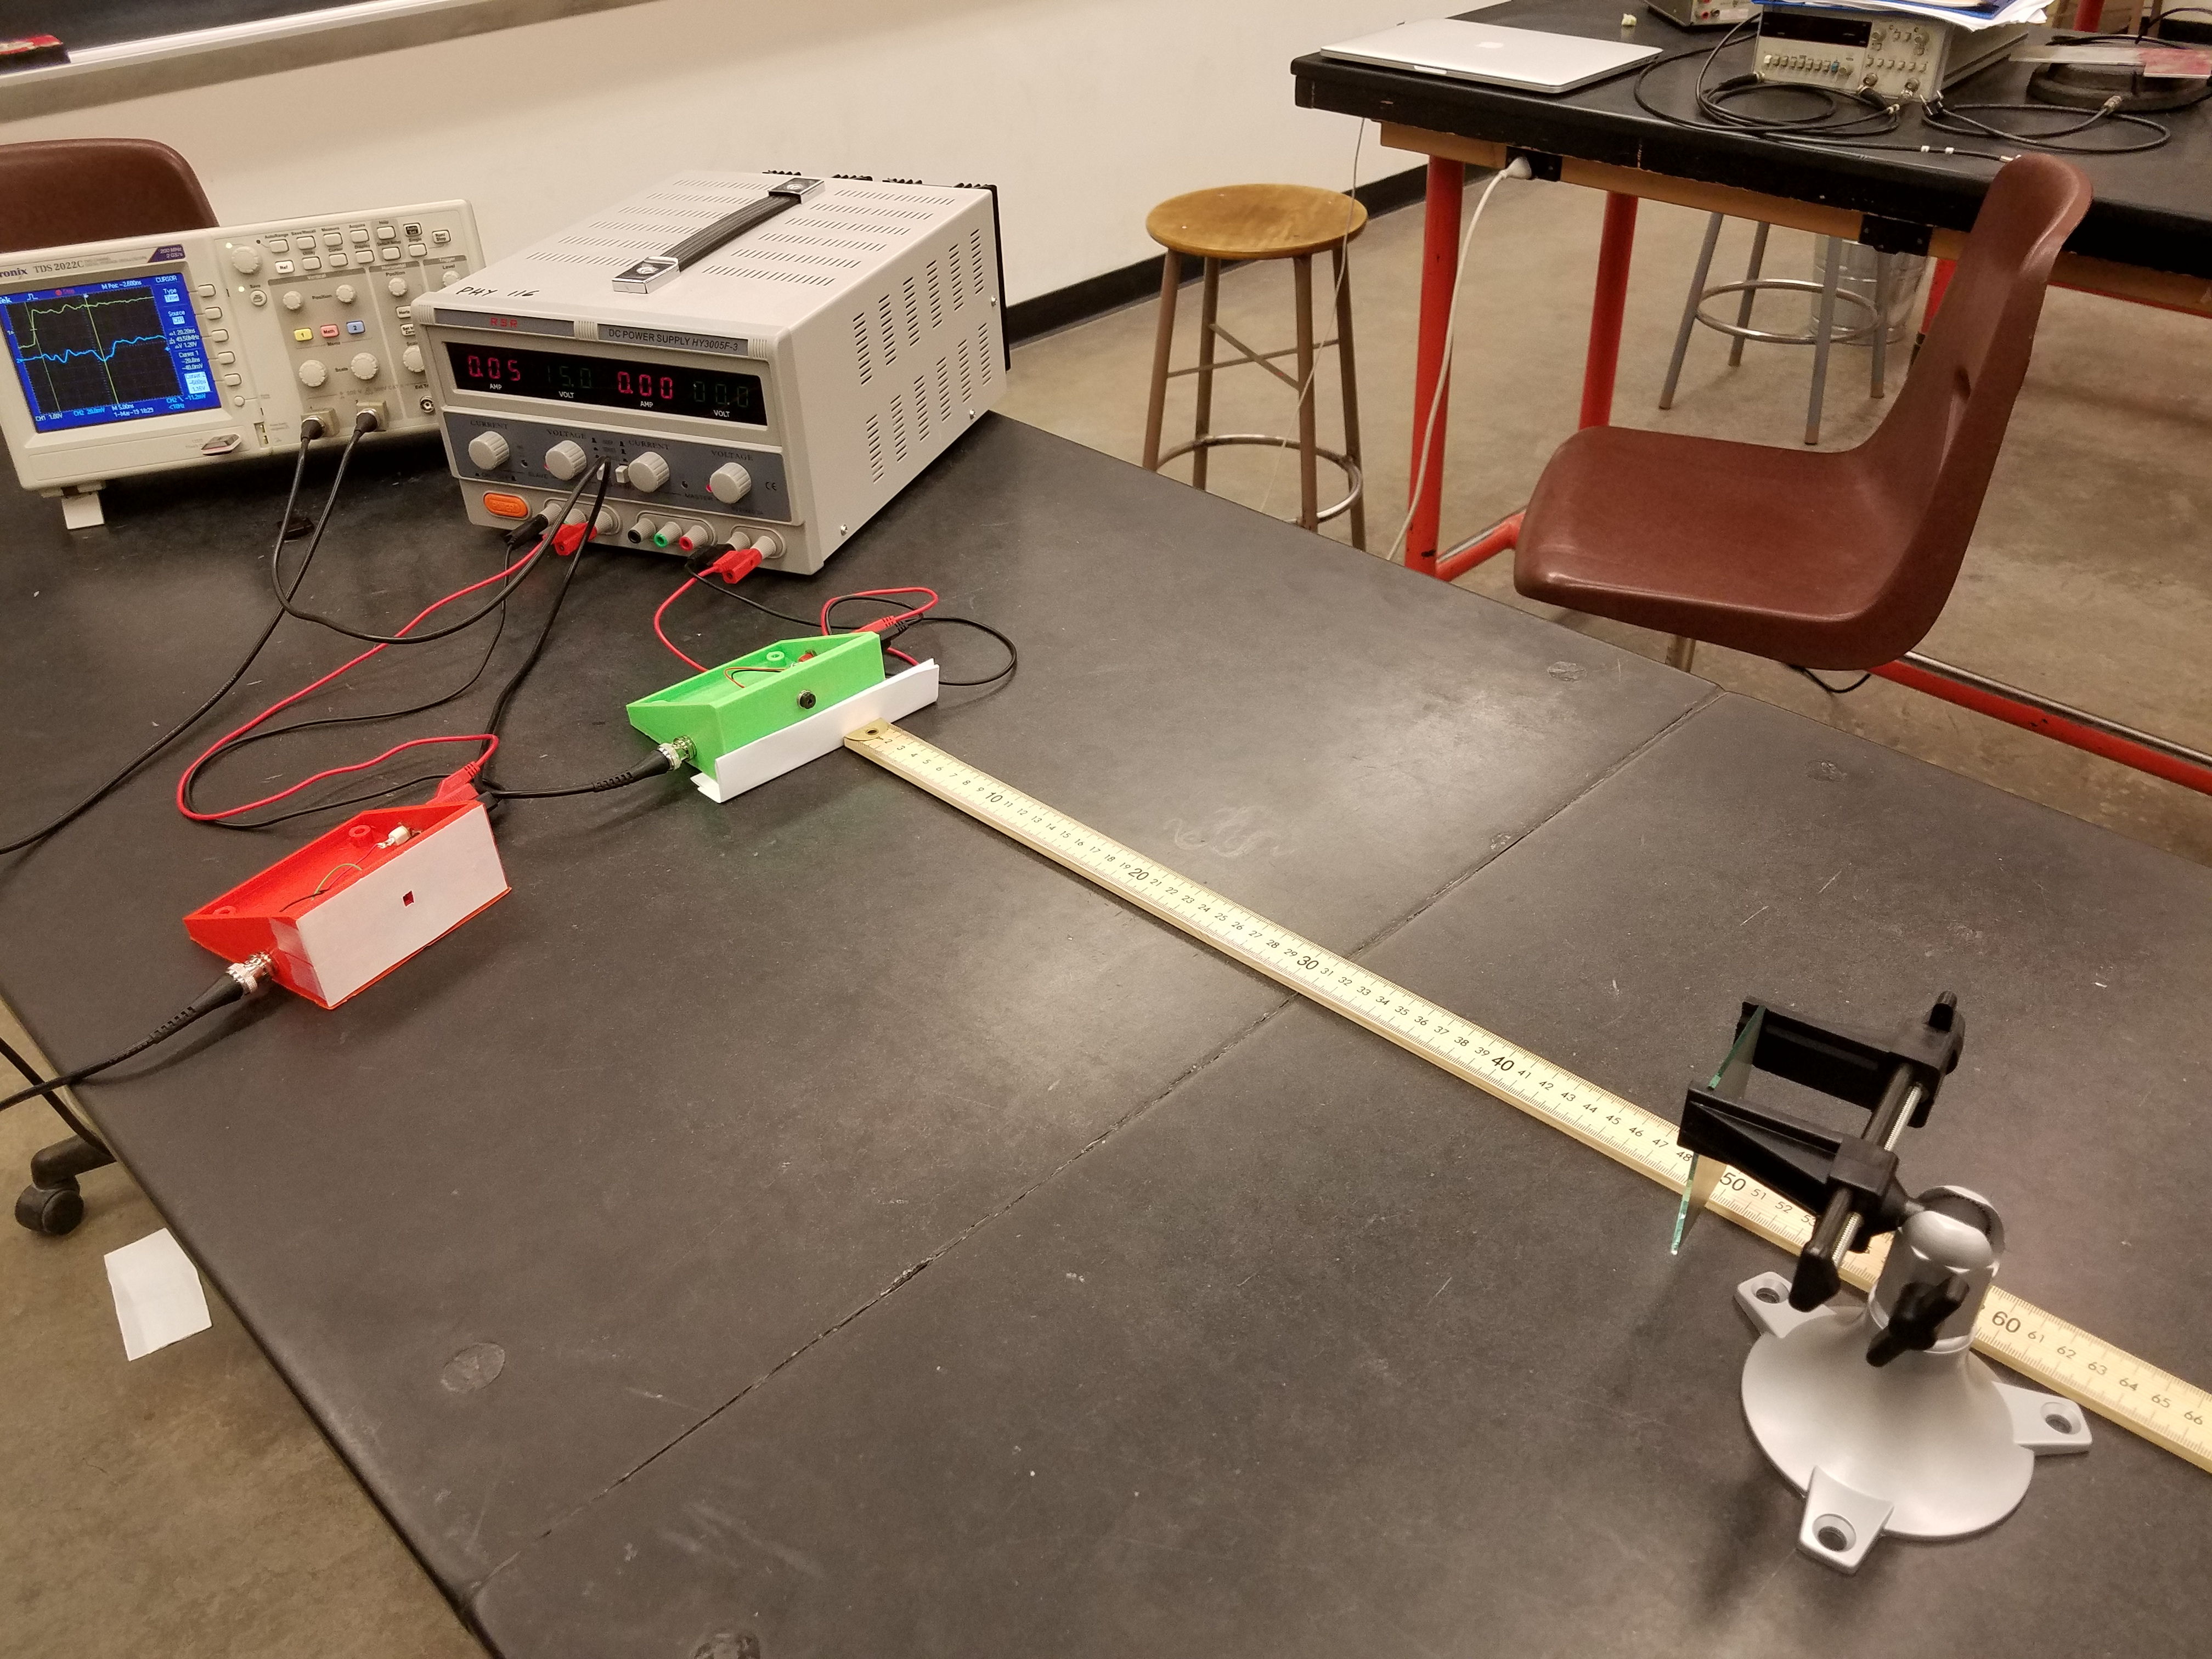
\includegraphics[height=0.25\textheight]{figs/labs/dc_circuits/setup.jpg} \\
(a) & (b) \\
\end{tabular}
\caption{Circuit for verifying Ohm's law as a (a) circuit diagram, and (b) implemented using your lab 
equipment.}
\label{fig:ohmslaw}
\end{center}
\end{figure}

Build the circuit in Fig.~\ref{fig:ohmslaw}.  Use a resistor $R_1 =
1.0~{\rm k\Omega}$ with a $1\%$ tolerance.  Use your Triplett 9007 as
the voltmeter and the Mastech MS8624 as the current meter.  Use your
benchtop power supply to provide the DC voltage.  Use banana plug
connectors for the current measurement, installing the Mastech MS8624
between the supply and the breadboard.

By adjusting the voltage setting of the power supply, take a series of
voltage and current measurements with voltage across the resistor at
target voltages from $1$ to $10~\rm V$ in steps of $1~\rm V$.
Generally, you can measure more precisely than you can control, so
never fuss about trying to measure the voltage at exactly the target
value, instead, simply record e.g. $V=1.04~\rm V$ along with your
current measurement and move on to the next target value.

While recording data, check that the current values you measure are
consistent with what you expect given the voltage across the resistor
and resistance.  You should {\em always} make quick sanity
calculations when collecting data, otherwise you risk wasting time
collecting useless data!

{\bf Plot 1:} Plot the current versus voltage of your ten data points
(using option {\tt "o"}).  Draw a line (using option {\tt "-"}) for
the current versus voltage curve of a $1.0~\rm k\Omega$ resistor.
Make certain your plot has appropriate axis labels, including
appropriate units in parenthesis, and a legend distinguishing data
from your expectation (``expected").  

{\bf Measurement 1:} After taking your last measurement, leave all the
connections in place and the power-supply at $10~\rm V$.  Record in
your log book the resistance of the resistor $R_1$ reported by your
DMM.  Is this a reasonable measurement?  {\bf Measurement 2:} Turn off
the DC supply and record the resistance reported by the DMM.  Is this
accurate?  {\bf Measurement 3:} Remove the resistor from your circuit
and measure the resistance with your DMM.  Is this accurate?

\section{Voltage Divider}
One circuit you will encounter again and again is the humble voltage
divider circuit of Fig.~\ref{fig:dividers} a.  Modify your setup to
include an additional resistor $R_2 = 4.7~\rm k\Omega$ in series with
your resistor $R_1 = ~\rm 1~\rm k\Omega$.  Before installing it in
your circuit, record the actual value of your resistor $R_2$ in your
log book.

{\bf Measurement 4:} adjust the supply voltage to $10~\rm V$ and
record the voltage across resistor $R_1$, the voltage across resistor
$R_2$, and the current through the divider.  Compare these measured
values to your expectation.

Now adjust your circuit so that $R_1$ and $R_2$ are in parallel and
set the supply to $10~\rm V$ {\bf Measurement 5:} Record the voltage
across the resistors $R_1$ and $R_2$ and the current through each
resistor.  Compare the measured currents to your expectation.

\begin{figure}[htbp]
\begin{center}
\begin{tabular}{c@{\hskip 2cm}c}
\begin{circuitikz}[line width=1pt]
\draw (0,0) to[voltage source,bipoles/length=1.5cm] ++(0,+4.0) to[short] ++(2.0,0);
\draw (A) to[resistor,l_=$R_1$] ++(0,-2.0) to[resistor,l_=$R_2$] ++(0,-2.0) to[short] ++(-2.0,0);
%node[ground,yscale=2.0]{};
\end{circuitikz} &
\begin{circuitikz}[line width=1pt]
\draw (0,0) to[voltage source,bipoles/length=1.5cm] ++(0,+4.0) to[short] ++(2.0,0) coordinate(A);
\draw (A) to[resistor,l_=$R_1$] ++(0,-4.0) to[short] ++(-2,0);
%node[ground,yscale=2.0]{};
\draw (A) to[short,*-] ++(2.0,0.0) to[resistor,l_=$R_2$] ++(0.0,-4.0) to[short,-*] ++(-2.0,0);
\end{circuitikz} \\
(a) & (b) \\
\end{tabular}
\caption{Circuits for studying resistors (a) in series, and (b) in parallel.}
\label{fig:dividers}
\end{center}
\end{figure}







